% Template for Cogsci submission with R Markdown

% Stuff changed from original Markdown PLOS Template
\documentclass[10pt, letterpaper]{article}

\usepackage{cogsci}
\usepackage{pslatex}
\usepackage{float}
\usepackage{caption}

% amsmath package, useful for mathematical formulas
\usepackage{amsmath}

% amssymb package, useful for mathematical symbols
\usepackage{amssymb}

% hyperref package, useful for hyperlinks
\usepackage{hyperref}

% graphicx package, useful for including eps and pdf graphics
% include graphics with the command \includegraphics
\usepackage{graphicx}

% Sweave(-like)
\usepackage{fancyvrb}
\DefineVerbatimEnvironment{Sinput}{Verbatim}{fontshape=sl}
\DefineVerbatimEnvironment{Soutput}{Verbatim}{}
\DefineVerbatimEnvironment{Scode}{Verbatim}{fontshape=sl}
\newenvironment{Schunk}{}{}
\DefineVerbatimEnvironment{Code}{Verbatim}{}
\DefineVerbatimEnvironment{CodeInput}{Verbatim}{fontshape=sl}
\DefineVerbatimEnvironment{CodeOutput}{Verbatim}{}
\newenvironment{CodeChunk}{}{}

% cite package, to clean up citations in the main text. Do not remove.
\usepackage{cite}

\usepackage{color}

% Use doublespacing - comment out for single spacing
%\usepackage{setspace}
%\doublespacing


% % Text layout
% \topmargin 0.0cm
% \oddsidemargin 0.5cm
% \evensidemargin 0.5cm
% \textwidth 16cm
% \textheight 21cm

\title{Arbitrariness and path dependence in a noisy-channel communication model}


\author{{\large \bf Robert Hawkins, Michael Frank, Noah Goodman} \\ \texttt{\{rxdh, mcfrank, ngoodman\}@stanford.edu} \\ Department of Psychology \\ Stanford University}

\begin{document}

\maketitle

\begin{abstract}


\textbf{Keywords:}
Add your choice of indexing terms or keywords; kindly use a semi-colon;
between each term.
\end{abstract}

\section{Introduction}\label{introduction}

Successful communication depends on a set of shared linguistic
conventions (de Saussure, XX; Lewis, XX). These conventions allow
communities of speakers to coordinate group behavior (cite collective
behavior lit??), initiate speech acts (Strawson, 1964), and align
beliefs or memories (Coman, Momennejad, Drach, \& Geana, 2016; Stolk,
Verhagen, \& Toni, 2016). While \emph{global} conventions adopted and
sustained throughout a large population of speakers may form over much
longer time scales (cite historical ling?), we also effortless
coordinate on \emph{ad hoc} or \emph{local} conventions -- or conceptual
pacts -- within the span of a single dialogue.

For instance, in a seminal study by Clark \& Wilkes-Gibbs (1986), pairs
of participants played an interactive reference game in which they were
separately presented with arrays of abstract tangram shapes in
randomized orders. One player -- the \emph{speaker} -- was instructed to
decribe the tangrams such that the other player -- the \emph{listener}
-- could rearrange their tangrams to accurately match the speaker's
board. Over six rounds, descriptions were dramatically shortened: an
early description like ``All right, the next one looks like a person
who's ice skating, except they're sticking two arms out in front''
became ``The ice skater'' by the final round.

In this paper, we present a probabilistic model of language
conventionalization in a communcation game. We show that this model,
based on recent successes capturing language understanding as social
inference (Goodman \& Frank, 2016; Goodman \& Stuhlmüller, 2013), can
account for key empirical signatures of conventions, including limited
arbitrariness, path-dependence, and systematic shortening over time.
These computational results are compared with qualitative empirical
results from a new large-scale replication of Clark \& Wilkes-Gibbs
(1986).

While simple evolutionary or agent-based models (Barr, 2004; Centola \&
Baronchelli, 2015; Shoham \& Tennenholtz, 1997; Young, 2015) have
previously been used to understand the dynamics of \emph{global}
conventions, relatively little modeling work has focused on the
cognitive mechanisms supporting emergence of conventions during shorter
dyadic interactions.

\begin{CodeChunk}
\captionsetup{width=0.8\columnwidth}\begin{figure}[H]

{\centering 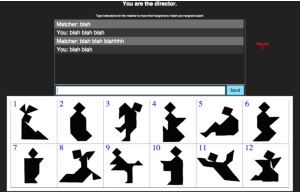
\includegraphics{figs/image-1} 

}

\caption{\label{fig:taskScreenshot} Example trial}\label{fig:image}
\end{figure}
\end{CodeChunk}

\section{Reference game experiment}\label{reference-game-experiment}

\subsection{Participants}\label{participants}

200 participants were recruited from Amazon's Mechanical Turk and paired
into dyads to play a reference game. We excluded X games because
participants reported confusion at the instructions, Y games because one
or both of the participants reported being a native language different
from English, and Z games for terminating early.

\subsection{Stimuli}\label{stimuli}

On every trial of the game, both participants were shown grid of twelve
tangram shapes, reproduced from (cite Herb; see Fig. \ref{fig:stimuli}).

\subsection{Procedure}\label{procedure}

After passing a short quiz about task instructions, participants were
randomly assigned the role of either `director' or `matcher' and
automatically paired into virtual rooms containing a chat box and grid
of stimuli. Both participants could freely use the chat box to
communicate, but only the matcher could click and drag stimuli to
reorder them. The director's goal was to tell the matcher\dots

\section{Acknowledgements}\label{acknowledgements}

Place acknowledgments (including funding information) in a section at
the end of the paper.

\section{References}\label{references}

\setlength{\parindent}{-0.1in} \setlength{\leftskip}{0.125in} \noindent

\hypertarget{refs}{}
\hypertarget{ref-Barr2004_ConventionalCommunicationSystems}{}
Barr, D. J. (2004). Establishing conventional communication systems: Is
common knowledge necessary? \emph{Cognitive Science}, \emph{28}(6),
937--962.

\hypertarget{ref-CentolaBaronchelli15_ConventionEmergence}{}
Centola, D., \& Baronchelli, A. (2015). The spontaneous emergence of
conventions: An experimental study of cultural evolution.
\emph{Proceedings of the National Academy of Sciences}, \emph{112}(7),
1989--1994.

\hypertarget{ref-ClarkWilkesGibbs86_ReferringCollaborative}{}
Clark, H. H., \& Wilkes-Gibbs, D. (1986). Referring as a collaborative
process. \emph{Cognition}, \emph{22}(1), 1--39.

\hypertarget{ref-ComanEtAl16_MnemonicConvergence}{}
Coman, A., Momennejad, I., Drach, R. D., \& Geana, A. (2016). Mnemonic
convergence in social networks: The emergent properties of cognition at
a collective level. \emph{Proceedings of the National Academy of
Sciences}, \emph{113}(29), 8171--8176.
\url{http://doi.org/10.1073/pnas.1525569113}

\hypertarget{ref-GoodmanFrank16_RSATiCS}{}
Goodman, N. D., \& Frank, M. C. (2016). Pragmatic language
interpretation as probabilistic inference. \emph{Trends in Cognitive
Sciences}, \emph{20}(11), 818--829.

\hypertarget{ref-GoodmanStuhlmuller13_KnowledgeImplicature}{}
Goodman, N. D., \& Stuhlmüller, A. (2013). Knowledge and implicature:
Modeling language understanding as social cognition. \emph{Topics in
Cognitive Science}, \emph{5}(1), 173--184.

\hypertarget{ref-ShohamTennenholtz97_EmergenceOfConventions}{}
Shoham, Y., \& Tennenholtz, M. (1997). On the emergence of social
conventions: Modeling, analysis, and simulations. \emph{Artificial
Intelligence}, \emph{94}(1), 139--166.

\hypertarget{ref-StolkVerhagenToni16_ConceptualAlignment}{}
Stolk, A., Verhagen, L., \& Toni, I. (2016). Conceptual alignment: How
brains achieve mutual understanding. \emph{Trends in Cognitive
Sciences}, \emph{20}(3), 180--191.

\hypertarget{ref-Strawson64_IntentionConvention}{}
Strawson, P. F. (1964). Intention and convention in speech acts.
\emph{The Philosophical Review}, 439--460.

\hypertarget{ref-Young15_EvolutionOfSocialNorms}{}
Young, H. P. (2015). The evolution of social norms. \emph{Annual Review
of Economics}, \emph{7}, 359--387.

\end{document}
